\documentclass[english]{article}
\usepackage{amsmath}
\usepackage{ae,aecompl}
\usepackage[T1]{fontenc}
\usepackage[latin9]{inputenc}
\usepackage{textcomp}
\usepackage{graphicx}
\usepackage{eurosym}
\usepackage[hidelinks]{hyperref}
\usepackage{float}
\usepackage{fancyhdr}
\usepackage{tabto}
\usepackage{verbatim}
\usepackage{etoolbox}
\usepackage[table]{xcolor}
\usepackage{booktabs}
\usepackage{wasysym}
\usepackage{multirow}
\usepackage{fancyhdr}
\usepackage{pdflscape}
\usepackage[scaled]{beramono}
\usepackage{csquotes}
\usepackage{comment}

\pagestyle{fancy}
\lhead{\powerenjoy I.T.P.D.}
\makeatletter
\makeatother
\usepackage{babel}

\newcommand\fnurl[2]{%
	\href{#2}{#1}\footnote{\url{#2}}%
}
\newcommand{\rent}{\textit{rent }}
\newcommand{\carsharing}{\textit {car sharing }}
\newcommand{\powerenjoy}{\textit{PowerEnjoy }}
\newcommand{\registereduser}{\textit {registered user }}
\newcommand{\registeredusers}{\textit {registered users }}
\newcommand{\powerenjoyuser}{\textit{PowerEnjoy User }}
\newcommand{\staff}{\textit{staff }}
\newcommand{\service}{\textit{service }}
\newcommand{\services }{\textit{services }}
\newcommand{\safearea}{\textit{safe area }}
\newcommand{\safeareas}{\textit{safe areas }}
\newcommand{\powerplug}{\textit{power plug }}
\newcommand{\powerplugs}{\textit{power plugs }}
\newcommand{\reservation}{\textit{reservation }}
\newcommand{\stand}{\textit{stand }}
\newcommand{\fieldstaff}{\textit{field staff }}
\newcommand{\resevation}{\textit{reservation }}
\newcommand{\stopover}{\textit{stopover }}
\newcommand{\personalpin}{\textit{personal pin }}
\newcommand{\guest}{\textit{guest }}
\newcommand{\thirdparty}{\textit{third party developer }}
\newcommand{\powerplugslot}{\textit{power plug slot }}
\newcommand{\moneysaving}{\textit{money saving }}
\begin{document}

	\begin{figure}
		\centering
		
\includegraphics[scale=0.5]{logo.pdf} 
	\end{figure}


	\title{PowerEnJoy\\
	Integration Test Plan Document\\
	}

	\date{A.A 2016/2017}
	
	\author{Erba Alessandro\\
	 Leveni Filippo\\
	 Lodi Luca}
	
	\maketitle
	\pagebreak{}
	\tableofcontents{} \pagebreak{}
\section{Introduction}
	\subsection{Revision History}
	
	\subsection{Purpose and Scope}
	This document will provide the guideline to accomplish the Integration test for the \powerenjoy service, it will provide specifically:
	\begin{itemize}
		\item the identification of the software components that are going to be integrated, with references to the Design Document according to the Requirement Analysis Specification Document.
		\item the organization of testing on subsystems in which \powerenjoy system is split.
		\item the schedule and description of the expected integration tests.
		\item the description of the used test tool.
	\end{itemize}
	\subsection{List of Definitions and Abbreviations}
	\subsubsection{Rent}
			A \rent is the activity beginning with the pick up and ending with the release of a car. It can include some \stopover.
		\subsubsection{Car Sharing}
			\carsharing is a model of car rental where people rent cars for short periods of time, often by the hour.
		\subsubsection{PowerEnJoy}
			\powerenjoy is the \carsharing brand object of this document.
		\subsubsection{Guest User}
			A \guest is a person not logged in to the system.
		\subsubsection{Registered User} 
			A \registereduser is a person registered to \powerenjoy.
		\subsubsection{PowerEnJoy User}
			A \powerenjoyuser is a \registereduser can access to the \carsharing through his smart device.
		\subsubsection{Staff}
			\staff is the set of people that are \registereduser  but can perform special operations. They are divided in three different categories.
			\begin{itemize}
				\item {Field \staff}
				\begin{itemize}
				\item They own a passepartout for cars reporting any issues \\ \par (e.g: cars with low battery).
				\end{itemize}
				\item{Emergency \staff}
				\begin{itemize}
				\item They manage users issues. They are able to directly contact users.
				\end{itemize}
				\item{Management \staff}
				\begin{itemize}
				\item They manage the system, configuring its parameters. They can add new \safeareas, modify \carsharing fares and create new \staff accounts.
				\end{itemize}
			\end{itemize}
		\subsubsection{Third Party Developer}
			\thirdparty is a person that can fulfill operations on \powerenjoy system via API.
		\subsubsection{Service}
			The \service is the group of actions that a \powerenjoyuser can fulfill trough his smart device.	
		\subsubsection {Safe Area}
			A \safearea is a  geographical place\footnote{defined by a set of geolocation positions} on the map in which parking is allowed. \safearea are saved into the system. A \rent can end parking the car only in safe areas.
	\subsubsection{Power Plug}
		A \powerplug is the station that charges the battery of an electric car. All \powerplugs are displayed in the map on-board \powerenjoy cars. Each \powerplug is in a \safearea. A \powerenjoyuser who plugs his car into a \powerplug receives a discount according to \powerenjoy rules.
	\subsubsection{Power Plug Slot}
		A \powerplugslot is a parking slot reserved for the \powerplug charge of cars.
	\subsubsection{Parking solution}
		Either a \safearea or a \powerplugslot.
	\subsubsection{Reservation}
		A \resevation is the action of booking a car, within an hour from its pick up.
	\subsubsection{Stopover}
		A \stopover is a temporary power-off of a rented car. During a \stopover the \powerenjoyuser can leave the car,  and re-unlock it later through his smart device. It is subject to a different fare than the rest of rent time.
	\subsubsection{Fare}
		A policy to compute price of a rent, complete of involved parameters. \par E.g: proportional to time, 0.67\euro/minute during active rent time 
	\subsubsection{Personal Identification Number (PIN)}
		 \personalpin is a number of 5 digits that the user inserts on the car screen to enable driving commands.
	\subsection{List of Reference Documents}
	\begin{thebibliography}{9}

		\bibitem{RASD}
			Erba A., Leveni F., Lodi L.,
  			\emph{Requirement Analysis Specification Document},
 			2016.
 			
		\bibitem{DD}
			 Erba A., Leveni F., Lodi L.,
  			\emph{Design Document},
 			2016.
	\end{thebibliography}
\section{Integration Strategy}
	\subsection{Entry Criteria}
	In order to make the Integration test feasible the following conditions must be verified before it begins.
		 \begin{itemize}
		 	\item Requirement Analysis and Specification Document and Design Document must be complete in each section and already approved.
		 	\item All the parts of the component required by an integration test must be implemented.
		 	\item All the tested component's sub-parts (related to an integration test) are unit-tested and bug free.
		 	\item A risk assessment must already be evaluated (for the Critical modules approach)
		 	\item Integration Test data set has already been selected.
		\end{itemize}
	Another  important thing that we assume as milestone at this point is that all the external services that we interact with are already been tested during unit test. The point is that is impossible to have correctly completed the unit test without interfacing with external services.
	\par Specifically the following components are already integrated: \textit{Push Notification Adapter, Google Maps Adapter, Car navigation Adapter, Car Controller, Document Validation Service Adapter, Payment Service Adapter.}
	\subsection{Elements to be Integrated}
	Given the component diagram at section 2.2 of the Design Document every component colored in Orange and Yellowish will be integrated.
	Specifically the components will be integrated among them following the interfaces that they share.
	\subsection{Integration Testing Strategy}
	Among all the different Integration Testing Strategy we have chosen an approach based on the Critical Modules. 
	\par Our System is quite complex, we have a lot of features that supports the core business. During our analysis we have decided to give a priority to certain requirements (reference to section 2.1.9 of RASD Document). Following this priority hierarchy we have the need to test integrations of components interfaces related to these requirements. 
	\par Following the section 5 (Requirements Traceability) of the Design Document we can easily identify which components interfaces are related to the priorities. 
	\par The components (grouped by priority) are ordered by the criticality for the project, following the risk assessment analysis suggestions, from the most risky to the least one.
	\par This means that given all the components of our system, we will sort them following the 2.1.9 RASD Priorities; than each group will be tested using critical modules approach from the riskiest module.	
	We chose this feature-oriented strategy to reduce the risk of project failure, since we have defined a rich set of feature in the previous documents, and also a priority for the introduction of those feature in the software roadmap.
	\subsection{Sequence of Component/Function Integration}
		Here we show how the integration test is organized using the strategy chosen above. 
		\par We have divided all the components in 3 subsystems. The three subsystems  are the one suggested by the priorities of paragraphs 2.1.9 of the RASD Document.
		\par Every subsystem is organized in levels that represents the criticality of the components that it contains. From top to down criticality decreases. 
		\par The criticality of each component is related to its complexity and importance. We have carefully analyzed what each component will provide and foresee the effort to fix  any possible error. 
		\par As already said each module interface is not tested all at once. Each test case will cover certain features. By the end of the integration test phase all the modules will be completely  covered.
		\par In the next section we will explain what each test will cover.
		\subsubsection{PowerEnJoy User related integration test}
			We have carefully examined the different priorities and we come up with this configuration for the test:
			\begin{enumerate}
				\item \textbf{BPM} 
				\item \textbf{Rent manager, Reservation Manager} 
				\item \textbf{\powerenjoy User Manager, Payment Manager}
				\item \textbf{Map Manager, Service Configuration, Account Manager} 
				\item \textbf{\powerenjoy mobile app} 
			\end{enumerate}
			in Figure~\ref{fig:powerenjoyuser} you can see the dependencies between components 
			\begin{figure}[H]
				\centering
				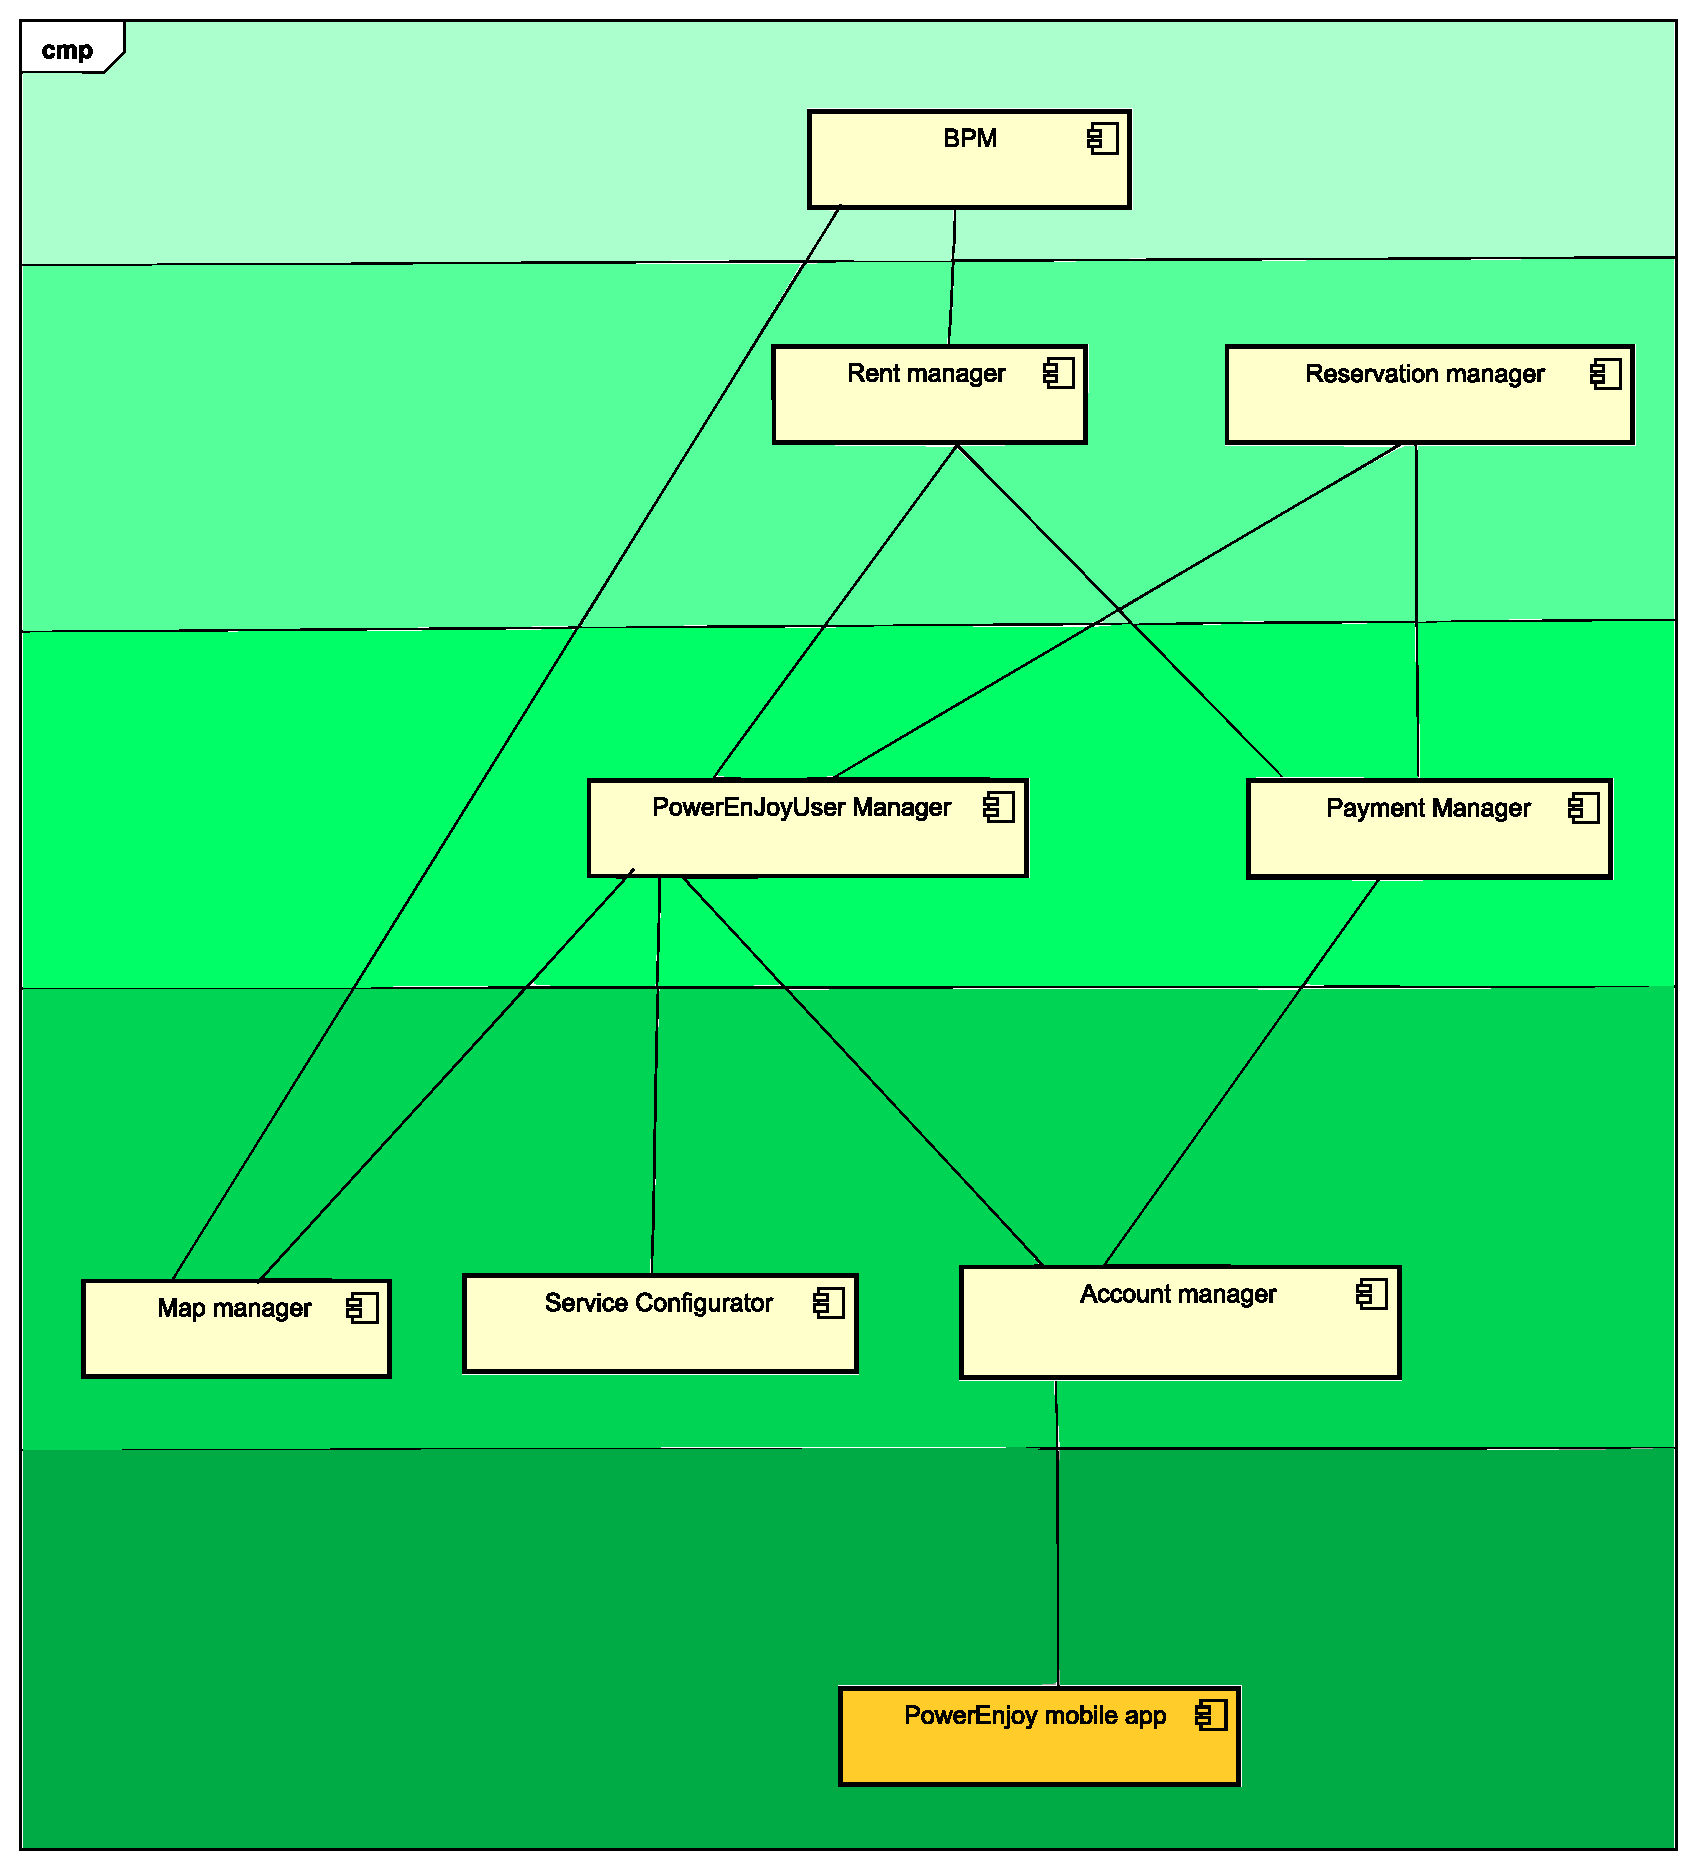
\includegraphics[scale=0.4]{./testingOrganization/powerenjoyuser.pdf}% "%" necessario
				\caption{PowerEnJoy User related integration test}
				\label{fig:powerenjoyuser}
			\end{figure}
			
		\subsubsection{Staff and Car related integration test}
			This integration test is divided in two, one about Emergency Staff, Field Staff and Cars Related Components;
			the second about Managements staff related components. This split is suggested by the related features of the first group, i.e. there was a high interaction of components of the three categories and it was more easy to group them together.
			
			We have carefully examined the different priorities and we come up with this configuration for the test:
			\begin{enumerate}
				\item \textbf{Car Manager} 
				\item \textbf{Emergency Staff manager, Field Staff Manger} 
				\item \textbf{Emergency Staff Web App, Field Staff mobile app,  Emergency manager, BPM, Map Manager}
				\item \textbf{Car App} 
			\end{enumerate}
			in Figure~\ref{fig:staffandcar} you can see the dependencies between components  
			\begin{figure}[H]
				\centering
				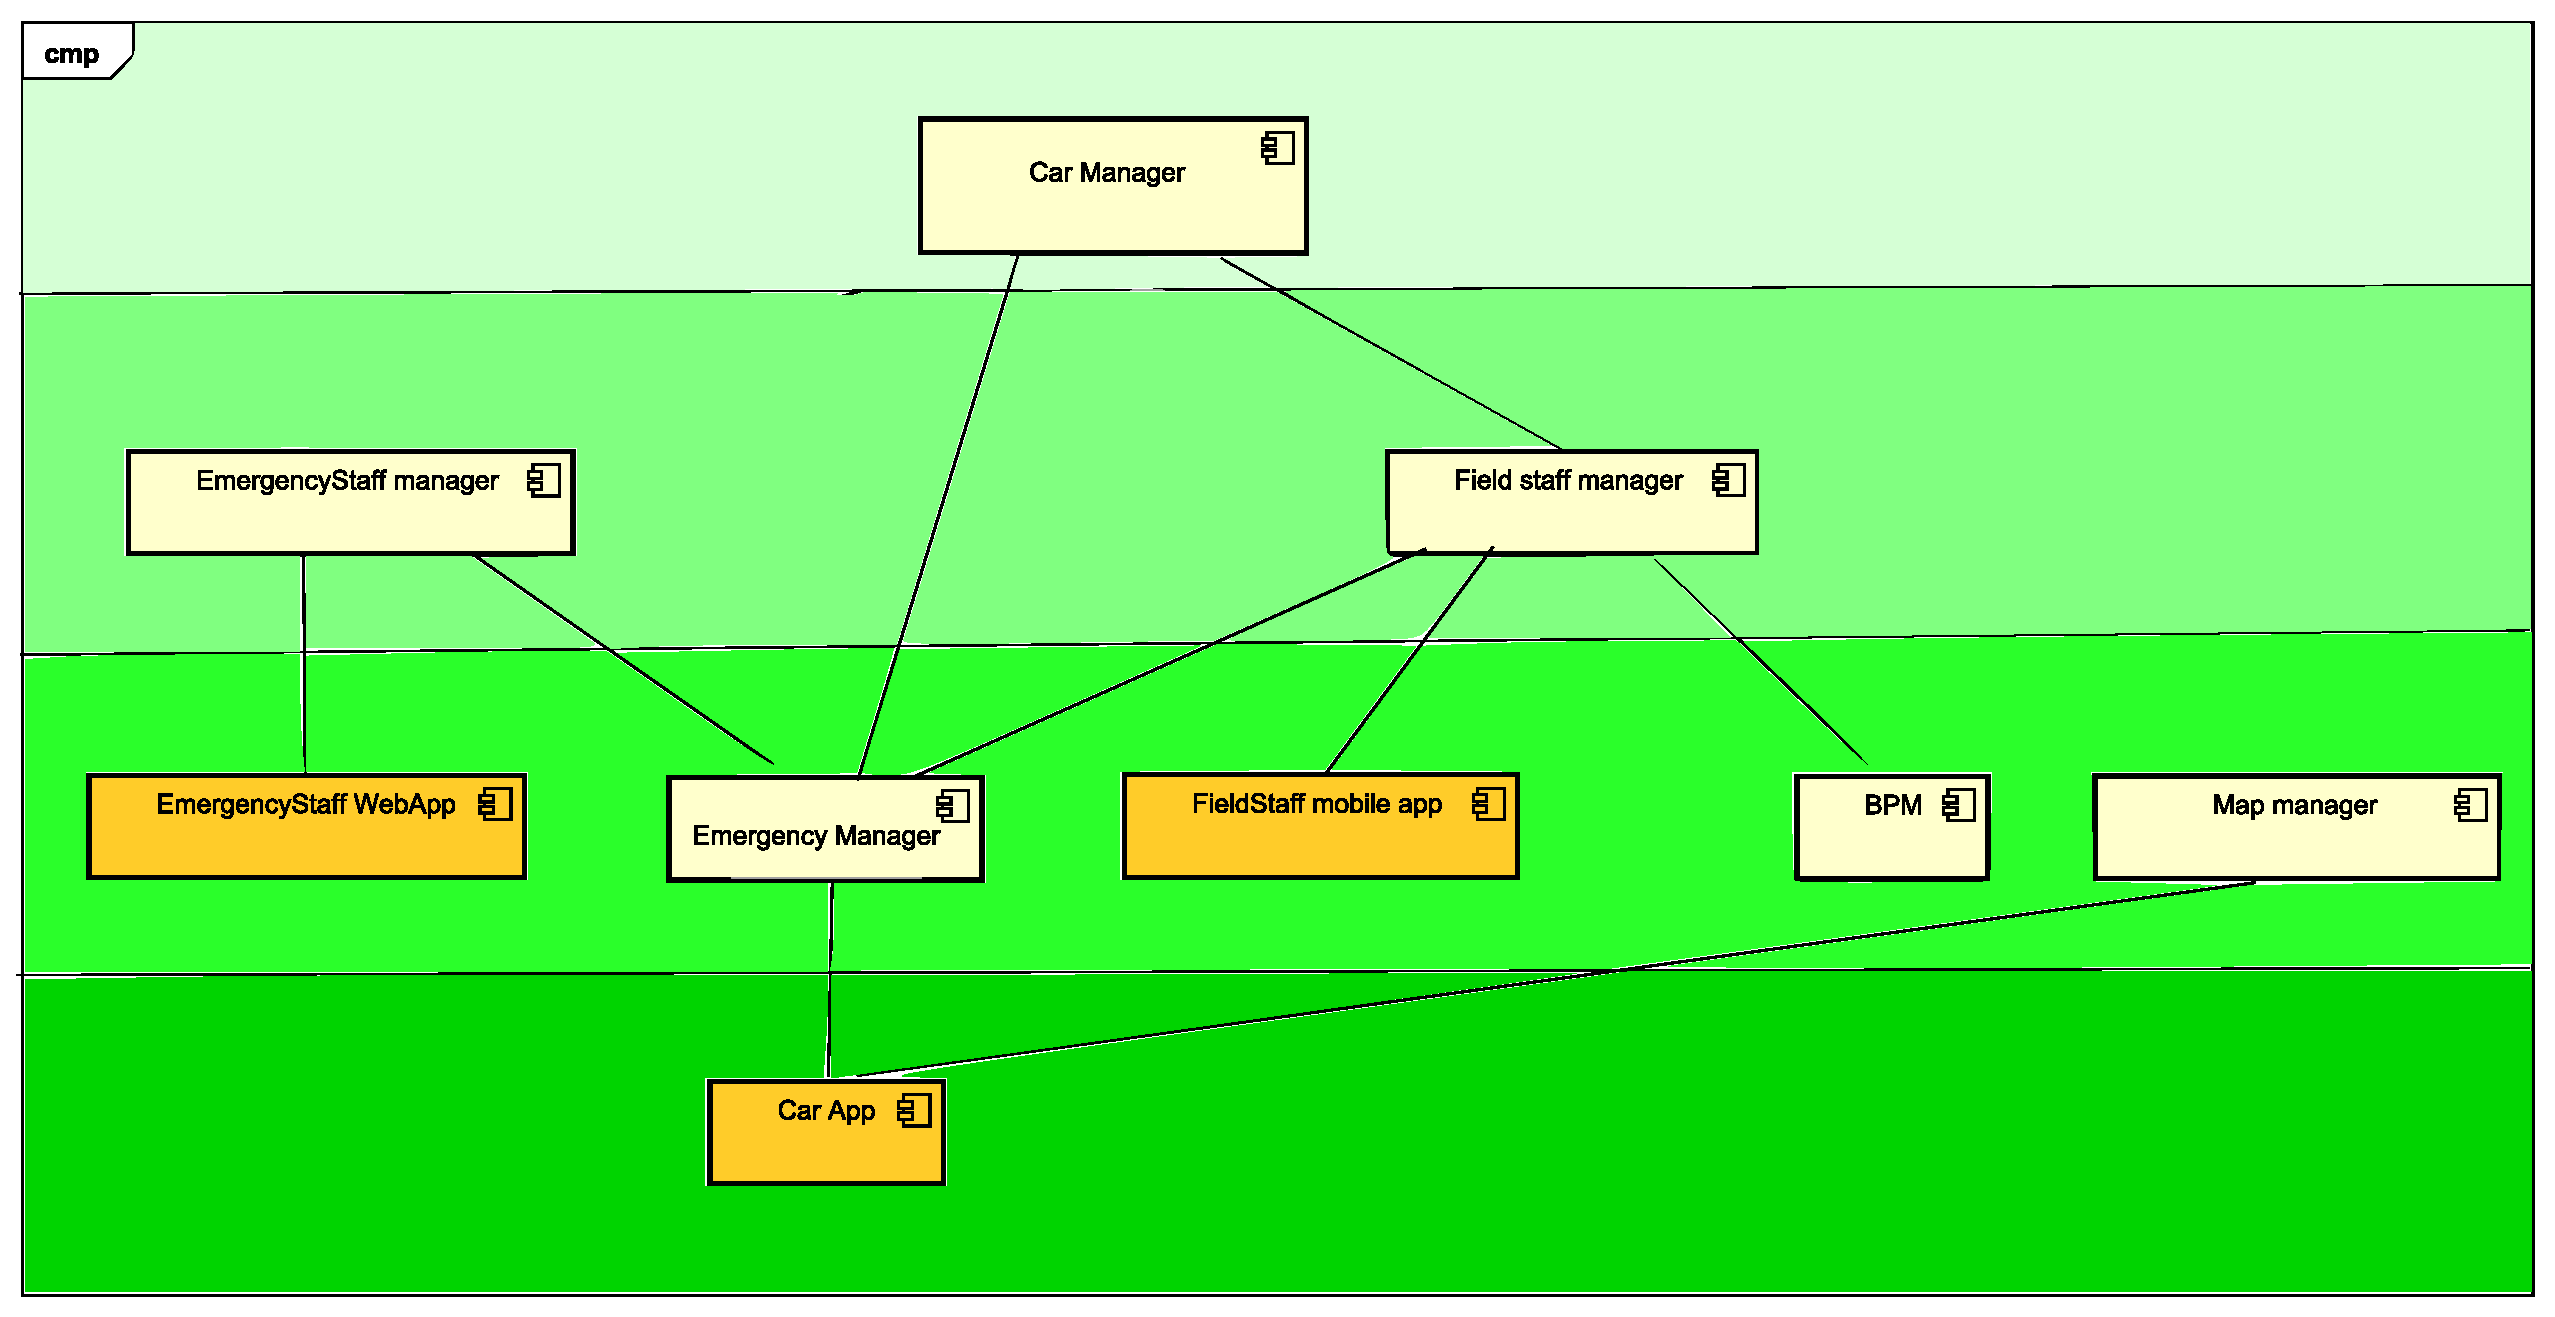
\includegraphics[scale=0.3]{./testingOrganization/staff_car.pdf}% "%" necessario
				\caption{Emergency Staff, Field Staff and Car related integration test}
				\label{fig:staffandcar}
			\end{figure}
			
			We have carefully examined the different priorities and we come up with this configuration for the test:
			\begin{enumerate}
				\item \textbf{Service Configurator} 
				\item \textbf{Management Staff Manager, PowerEnjoy User Manger} 
				\item \textbf{Management Staff Web App, BPM, Rent manager, Reservation Manager}
			\end{enumerate}
			
			in Figure~\ref{fig:managementstaff} you can see the dependencies between components  
			\begin{figure}[H]
				\centering
				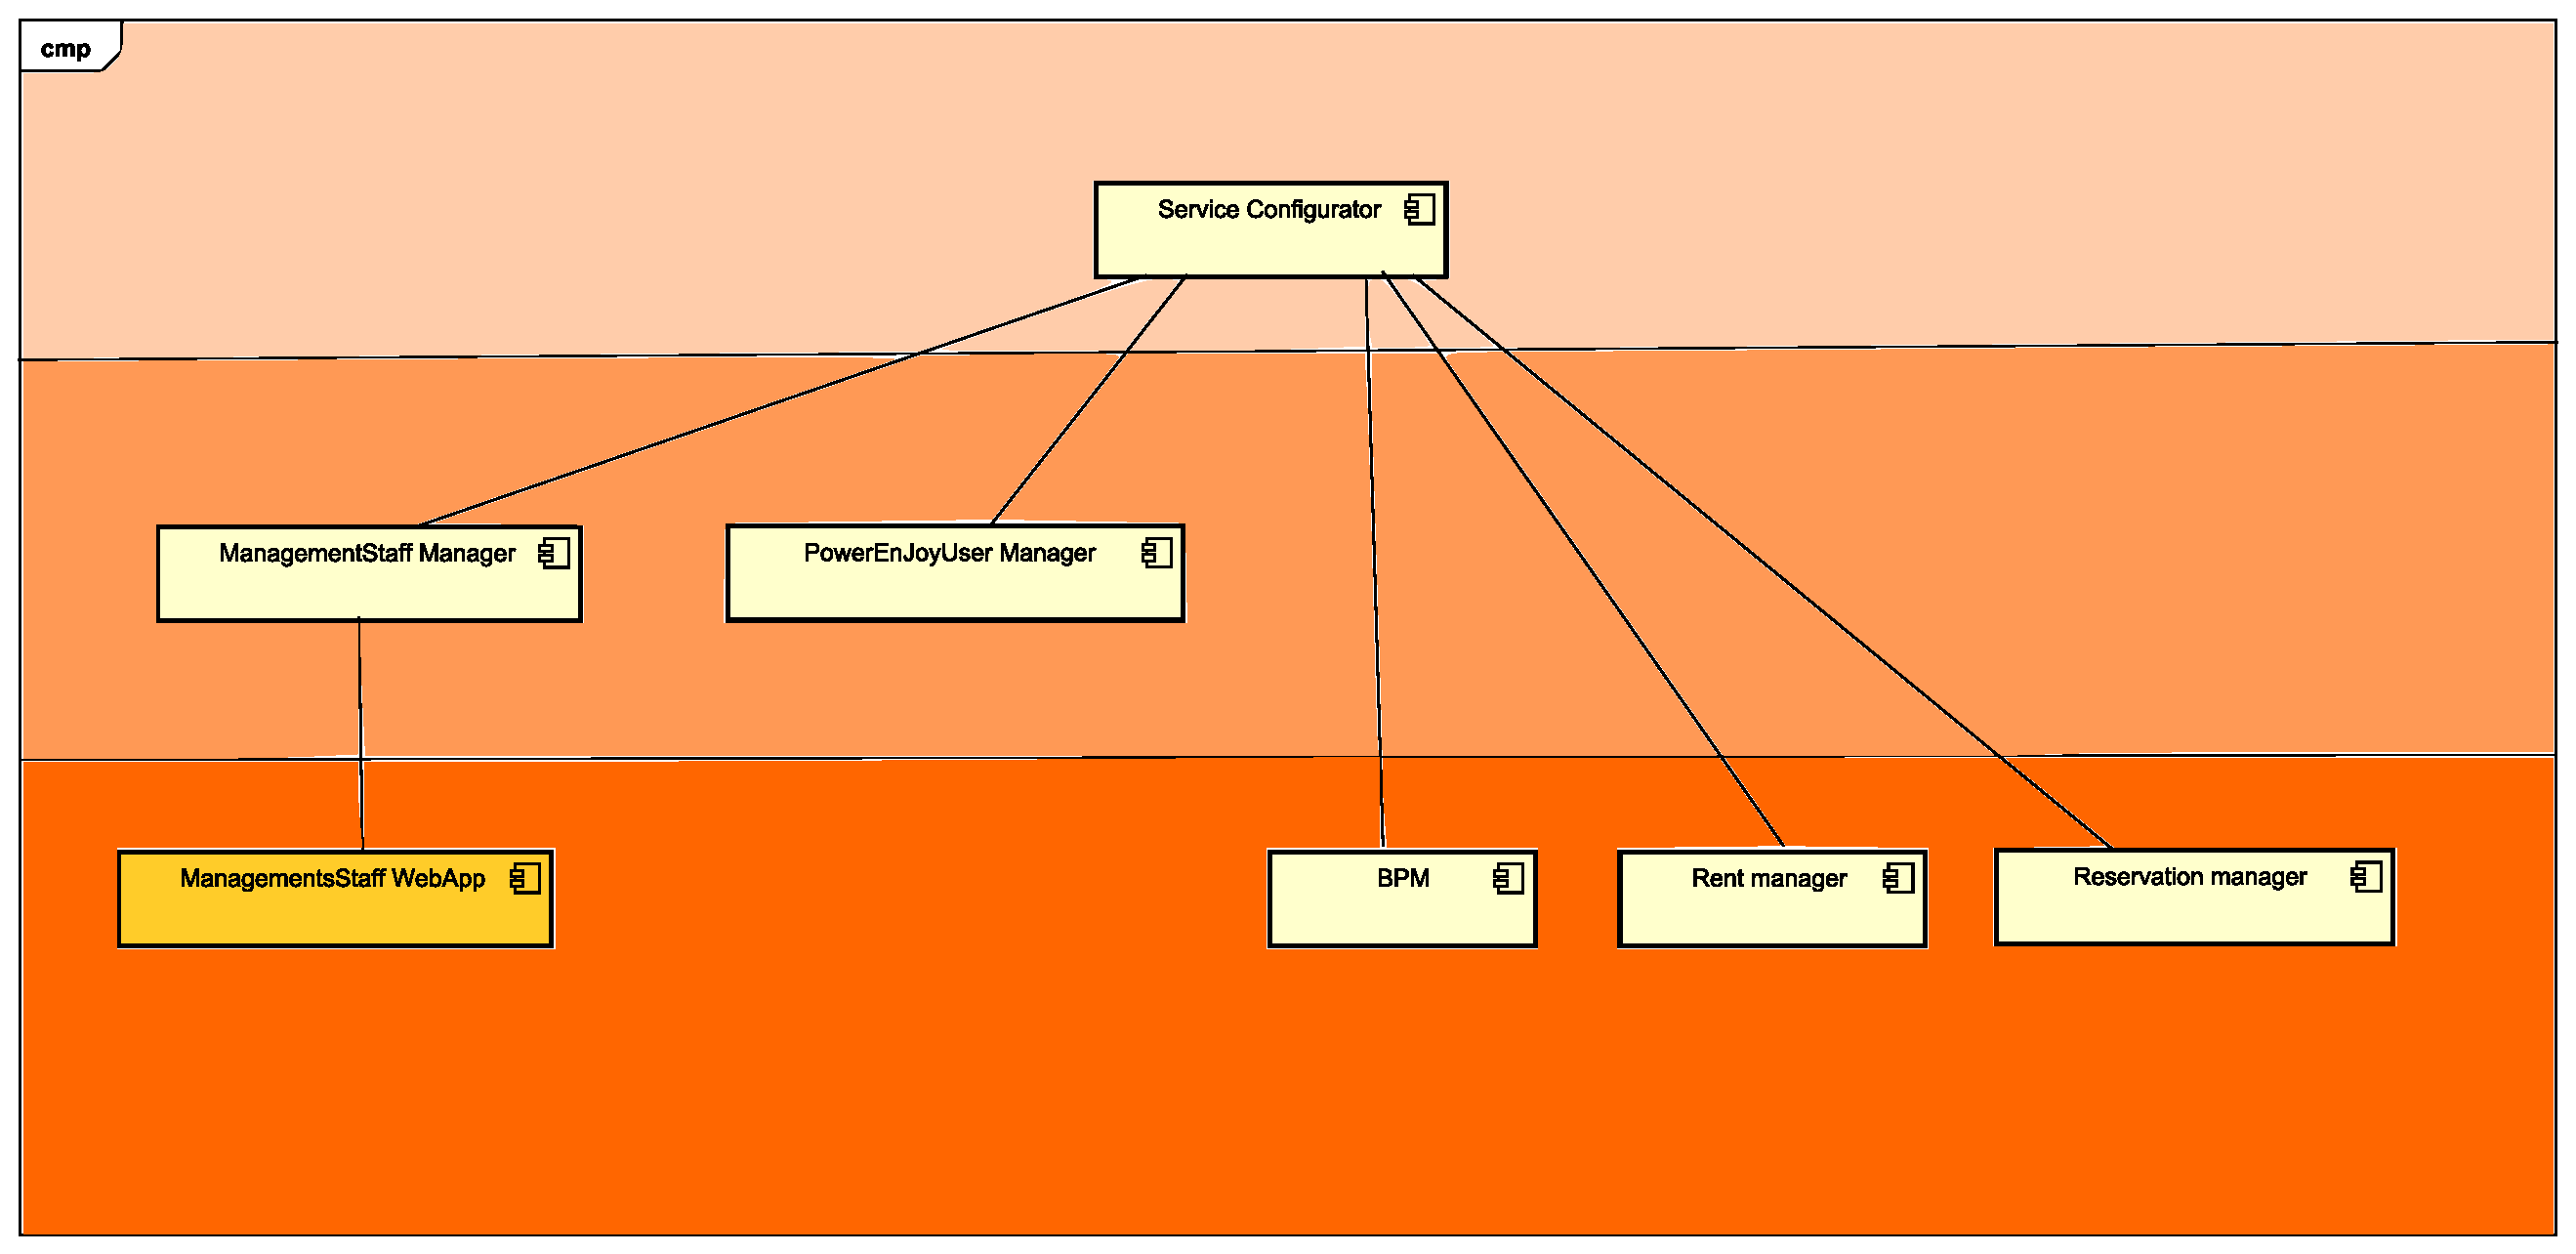
\includegraphics[scale=0.3]{./testingOrganization/managementstaff.pdf}% "%" necessario
				\caption{Management Staff related integration test}
				\label{fig:managementstaff}
			\end{figure}
		
		\subsubsection{Third Party related integration test}
		       We have carefully examined the different priorities and we come up with this configuration for the test:
			\begin{enumerate}
				\item \textbf{External App Manager} 
				\item \textbf{Account Manager PowerEnjoy User Manager} 
				\item \textbf{Map Manager, Rent manager, Reservation Manager}
			\end{enumerate}
			
			in Figure~\ref{fig:externalappmanager} you can see the dependencies between components 
			\begin{figure}[H]
				\centering
				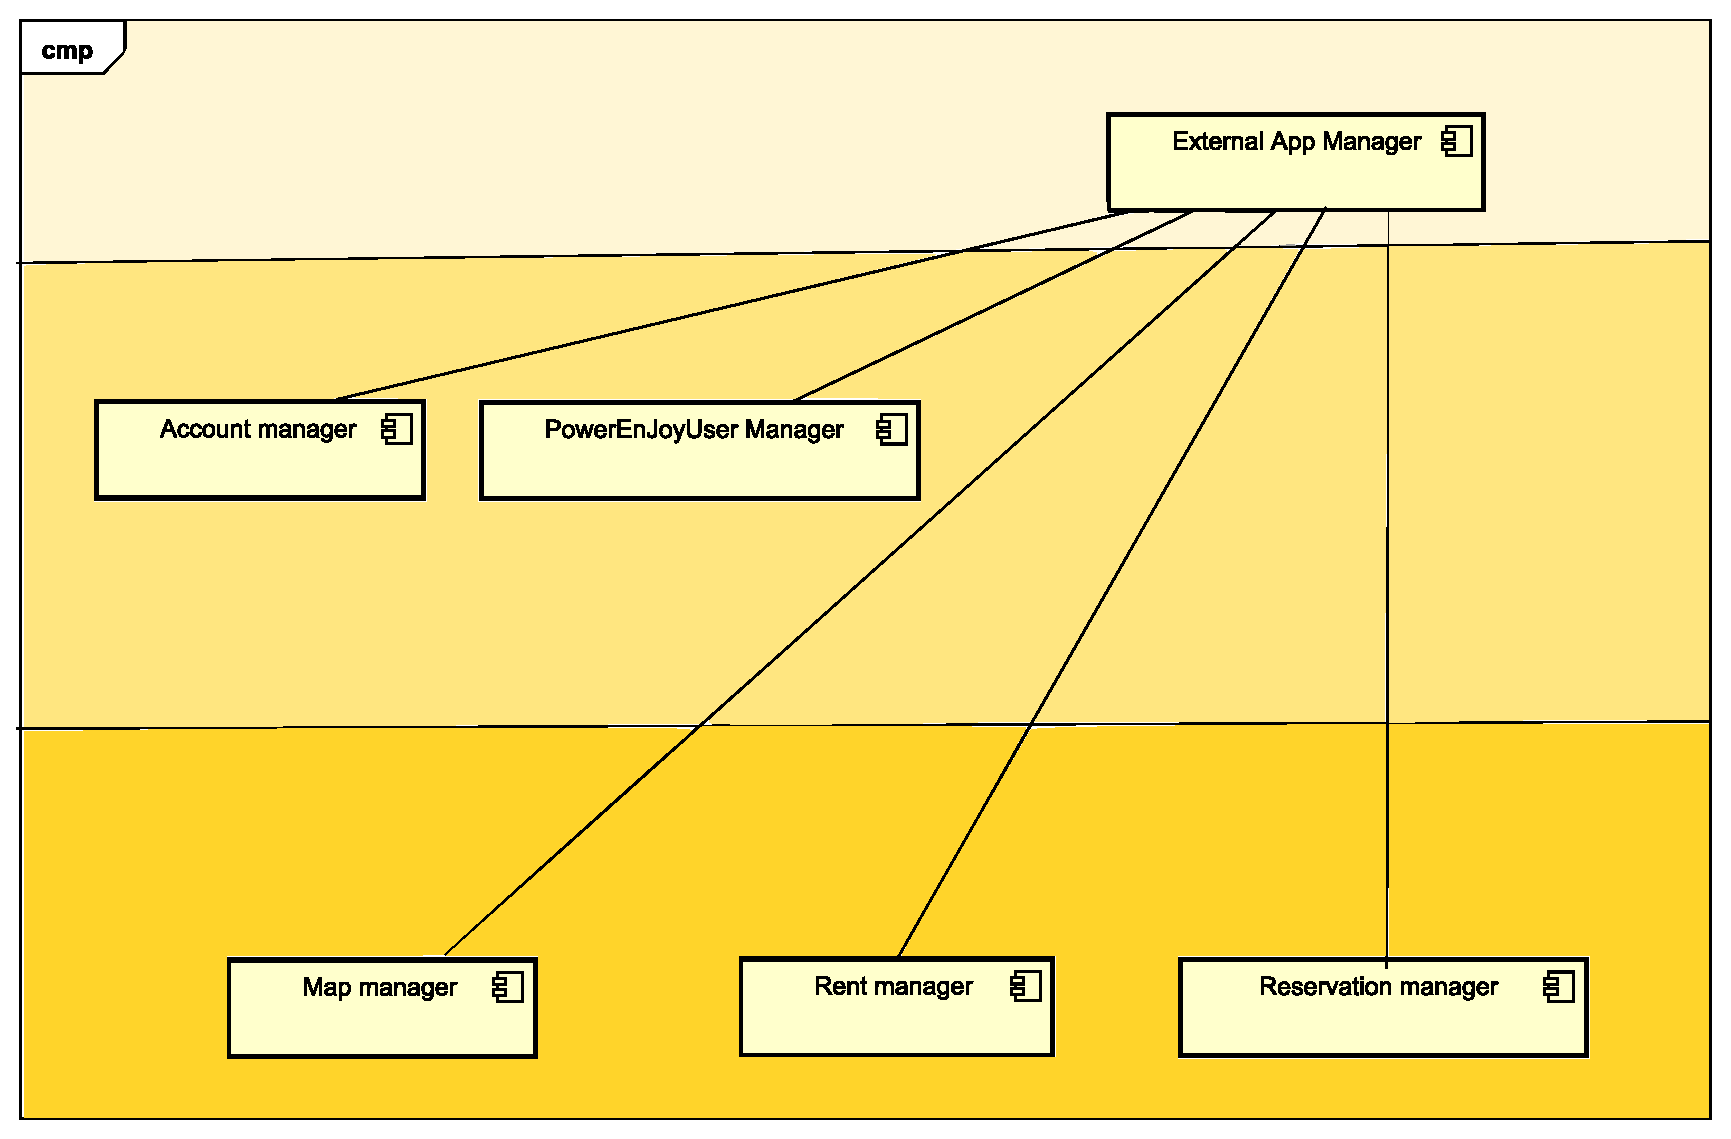
\includegraphics[scale=0.4]{./testingOrganization/externalappmanager.pdf}% "%" necessario
				\caption{Third Party related integration test}
				\label{fig:externalappmanager}
			\end{figure}
\section{Individual Steps and Test Description}

 In this paragraph we are going to give an high-level description of the integration tests that will be performed on PowerEnJoy system.
Since we adopted the critical modules strategy (feature-oriented approach), we do not have to worry about the heavy creation of drivers nor stubs. But we need to ``mock''  the component's classes not related to the tested interfaces, since they could be not already implemented. 
\par Following the critical module approach, we test the integration of couples of components (the sub-part related to the tested functionality) at a time, in order to find errors as soon as possible in the riskiest modules.

\par The following tables are structured as:
\begin{itemize}
\item{ \textbf{Test Case ID:} a label to identify the integration test under analysis.}
\item{ \textbf{Test Items:} the couple of involved components; \textquote{used by} relationship is represented through an arrow.}
\item{ \textbf{Input Specification:} the high-level description of the input (coming from
the right element of the item's couple previously specified)}
\item{ \textbf{Output Specification:} the high-level description of the expected output
provided the input above described.}
\item{ \textbf{Environmental Needs:} test execution's conditions, in terms of:
 \begin{itemize}
 \item{already performed tests}
 \item{already implemented functionalities}
 \end{itemize}}
\end{itemize}

\par NOTE:  For example in order to test the integration of BPM and Map manager (they interact through the \textquote{Map search API} interface), just a sub-part of those two components need to be already implemented. The unimplemented part of the two components need to be ``mocked'' (using mockito tool).  This apply to all the test cases described in the tables below.
			
			\begin{figure}[H]
				\centering
				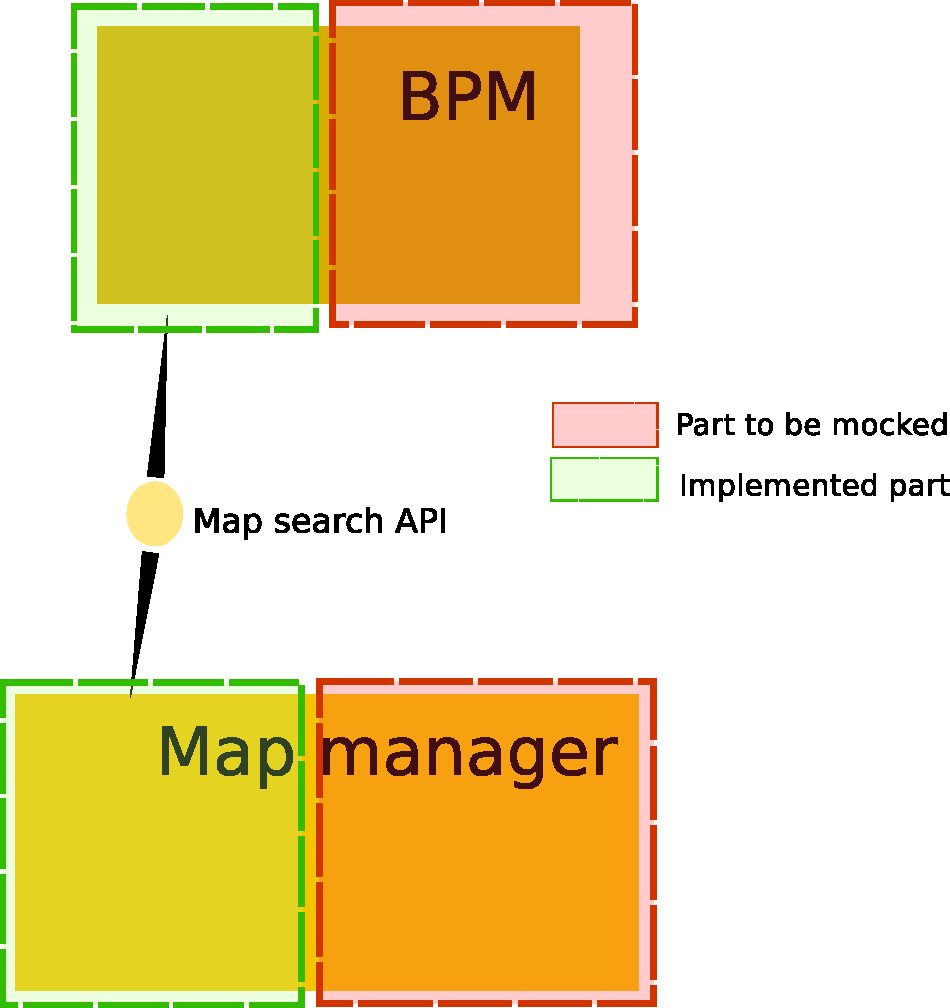
\includegraphics[scale=0.4]{./testingOrganization/example.pdf}% "%" necessario
				\caption{Integration example}
			\end{figure}



\subsection{PowerEnJoy User related integration tests}

\subsubsection{BPM integration test}

\begin{table}[H]
\centering
\begin{tabular}{|l|p{7cm}|}
\hline
 \textbf{Test Case ID} & I1-T1 \\ \hline 
 \textbf{Test Items} &  BPM ---> Map manager  \\ \hline
 \textbf{Input Specification} & a simulation of the typical BPM component input coming from Map manager, attention must be paid to cover the edge or exceptional cases related to the \textquote{Map search API} interface \\ \hline
 \textbf{Output Specification} & Check whether the correct methods are invoked, along with the correctness of the parameter types
and values \\ \hline
 \textbf{Environmental Needs} & The \textquote{Map search API} interface must have been already implemented and unit-tested  \\ \hline
\end{tabular}
\end{table}

\begin{table}[H]
\centering
\begin{tabular}{|l|p{7cm}|}
\hline
 \textbf{Test Case ID} & I1-T2 \\ \hline
 \textbf{Test Items} & Rent manager ---> BPM \\ \hline
 \textbf{Input Specification} & a simulation of the typical Rent manager component input coming from
BPM, attention must be paid to cover the edge or exceptional cases related to the \textquote{Recommend destination} interface \\ \hline
 \textbf{Output Specification} & Check whether the correct methods are invoked, along with the correctness of the parameter types
and values \\ \hline
 \textbf{Environmental Needs} & The \textquote{Recommend destination} interface must have been already implemented and unit-tested AND I1-T1 must have
already been performed \\ \hline
\end{tabular}
\end{table}

\subsubsection{Rent manager integration test}
\begin{table}[H]
\centering
\begin{tabular}{|l|p{7cm}|}
\hline
 \textbf{Test Case ID} & I2-T1 \\ \hline
 \textbf{Test Items} & PowerEnJoyUser manager ---> Rent manager \\ \hline
 \textbf{Input Specification} & a simulation of the typical PowerEnJoyUser manager component input coming from
Rent manager, attention must be paid to cover the edge or exceptional cases related to the \textquote{Rent API} interface \\ \hline
 \textbf{Output Specification} & Check whether the correct methods are invoked, along with the correctness of the parameter types
and values \\ \hline
 \textbf{Environmental Needs} & The \textquote{Rent API}  interface must have been already implemented and unit-tested AND I1-T2  must have
already been performed \\ \hline
\end{tabular}
\end{table}

\begin{table}[H]
\centering
\begin{tabular}{|l|p{7cm}|}
\hline
 \textbf{Test Case ID} & I2-T2 \\ \hline
 \textbf{Test Items} & Rent manager ---> Payment manager \\ \hline
 \textbf{Input Specification} & a simulation of the typical Rent manager component input coming from
Payment manager, attention must be paid to cover the edge or exceptional cases related to the \textquote{Payment transaction API}  interface \\ \hline
 \textbf{Output Specification} & Check whether the correct methods are invoked, along with the correctness of the parameter types
and values \\ \hline
 \textbf{Environmental Needs} & The  \textquote{Payment transaction API}  interface must have been already implemented and unit-tested \\ \hline
\end{tabular}
\end{table}

\subsubsection{Reservation manager integration test}
\begin{table}[H]
\centering
\begin{tabular}{|l|p{7cm}|}
\hline
 \textbf{Test Case ID} & I3-T1 \\ \hline
 \textbf{Test Items} & PowerEnJoyUser manager ---> Reservation manager \\ \hline
 \textbf{Input Specification} & a simulation of the typical PowerEnJoyUser manager component input coming from
Reservation manager, attention must be paid to cover the edge or exceptional cases related to the  \textquote{Reservation API}  interface \\ \hline
 \textbf{Output Specification} & Check whether the correct methods are invoked, along with the correctness of the parameter types
and values \\ \hline
 \textbf{Environmental Needs} & The  \textquote{Reservation API}  interface must have been already implemented and unit-tested \\ \hline
\end{tabular}
\end{table}

\begin{table}[H]
\centering
\begin{tabular}{|l|p{7cm}|}
\hline
 \textbf{Test Case ID} & I3-T2 \\ \hline
 \textbf{Test Items} & Reservation manager ---> Payment manager \\ \hline
 \textbf{Input Specification} & a simulation of the typical Reservation manager component input coming from
Payment manager, attention must be paid to cover the edge or exceptional cases related to the  \textquote{Payment transaction API}  interface \\ \hline
 \textbf{Output Specification} & Check whether the correct methods are invoked, along with the correctness of the parameter types
and values \\ \hline
 \textbf{Environmental Needs} & The  \textquote{Payment transaction API}  interface must have been already implemented and unit-tested \\ \hline
\end{tabular}
\end{table}


\subsubsection{PoweEnJoyUser manager integration test}
\begin{table}[H]
\centering
\begin{tabular}{|l|p{7cm}|}
\hline
 \textbf{Test Case ID} & I4-T1 \\ \hline
 \textbf{Test Items} & PowerEnJoyUser manager ---> Map manager \\ \hline
 \textbf{Input Specification} & a simulation of the typical PowerEnJoyUser manager component input coming from
Map manager, attention must be paid to cover the edge or exceptional cases related to the \textquote{Map search API} interface \\ \hline
 \textbf{Output Specification} & Check whether the correct methods are invoked, along with the correctness of the parameter types
and values \\ \hline
 \textbf{Environmental Needs} & The \textquote{Map search API} interface must have been already implemented and unit-tested \\ \hline
\end{tabular}
\end{table}

\begin{table}[H]
\centering
\begin{tabular}{|l|p{7cm}|}
\hline
 \textbf{Test Case ID} & I4-T2 \\ \hline
 \textbf{Test Items} & PowerEnJoyUser manager ---> Service configurator \\ \hline
 \textbf{Input Specification} & a simulation of the typical PowerEnJoyUser manager component input coming from
Service configurator, attention must be paid to cover the edge or exceptional cases related to the \textquote{Notification API} interface \\ \hline
 \textbf{Output Specification} & Check whether the correct methods are invoked, along with the correctness of the parameter types
and values \\ \hline
 \textbf{Environmental Needs} & The \textquote{Notification API} interface must have been already implemented and unit-tested  \\ \hline
\end{tabular}
\end{table}

\begin{table}[H]
\centering
\begin{tabular}{|l|p{7cm}|}
\hline
 \textbf{Test Case ID} & I4-T3 \\ \hline
 \textbf{Test Items} & PowerEnJoyUser manager ---> Account manager \\ \hline
 \textbf{Input Specification} & a simulation of the typical PowerEnJoyUser manager component input coming from
Account manager, attention must be paid to cover the edge or exceptional cases related to the \textquote{Registration API} interface \\ \hline
 \textbf{Output Specification} & Check whether the correct methods are invoked, along with the correctness of the parameter types
and values \\ \hline
 \textbf{Environmental Needs} & The \textquote{Registration API} interface must have been already implemented and unit-tested \\ \hline
\end{tabular}
\end{table}


\subsubsection{Payment manager integration test}
\begin{table}[H]
\centering
\begin{tabular}{|l|p{7cm}|}
\hline
 \textbf{Test Case ID} & I5-T1 \\ \hline
 \textbf{Test Items} & Payment manager ---> Account manager \\ \hline
 \textbf{Input Specification} & a simulation of the typical Payment manager component input coming from
Account manager, attention must be paid to cover the edge or exceptional cases related to the \textquote{Account API} interface \\ \hline
 \textbf{Output Specification} & Check whether the correct methods are invoked, along with the correctness of the parameter types
and values \\ \hline
 \textbf{Environmental Needs} & The \textquote{Account API} interface must have been already implemented and unit-tested \\ \hline
\end{tabular}
\end{table}

\subsubsection{Account manager integration test}
\begin{table}[H]
\centering
\begin{tabular}{|l|p{7cm}|}
\hline
 \textbf{Test Case ID} & I6-T1 \\ \hline
 \textbf{Test Items} & PowerEnJoyUser webapp ---> Account manager \\ \hline
 \textbf{Input Specification} & a simulation of the typical PowerEnJoyUser webapp component input coming from
Account manager, attention must be paid to cover the edge or exceptional cases related to the \textquote{Login API} interface \\ \hline
 \textbf{Output Specification} & Check whether the correct methods are invoked, along with the correctness of the parameter types
and values \\ \hline
 \textbf{Environmental Needs} & The \textquote{Login API} interface must have been already implemented and unit-tested \\ \hline
\end{tabular}
\end{table}


\subsection{Staff and Car related integration tests}

\subsubsection{Car manager integration test}
\begin{table}[H]
\centering
\begin{tabular}{|l|p{7cm}|}
\hline
 \textbf{Test Case ID} & I7-T1 \\ \hline
 \textbf{Test Items} & Car manager ---> Emergency manager \\ \hline
 \textbf{Input Specification} & a simulation of the typical Car manager component input coming from
Emergency manager, attention must be paid to cover the edge or exceptional cases related to the \textquote{Availability int} interface \\ \hline
 \textbf{Output Specification} & Check whether the correct methods are invoked, along with the correctness of the parameter types
and values \\ \hline
 \textbf{Environmental Needs} & The \textquote{Availability int} interface must have been already implemented and unit-tested \\ \hline
\end{tabular}
\end{table}

\begin{table}[H]
\centering
\begin{tabular}{|l|p{7cm}|}
\hline
 \textbf{Test Case ID} & I7-T2 \\ \hline
 \textbf{Test Items} & FieldStaff manager ---> Car manager \\ \hline
 \textbf{Input Specification} & a simulation of the typical FieldStaff manager component input coming from
Car manager, attention must be paid to cover the edge or exceptional cases related to the  \textquote{Car int} interface \\ \hline
 \textbf{Output Specification} & Check whether the correct methods are invoked, along with the correctness of the parameter types
and values \\ \hline
 \textbf{Environmental Needs} & The \textquote{Car int} interface must have been already implemented and unit-tested \\ \hline
\end{tabular}
\end{table}

\subsubsection{EmergencyStaff manager integration test}
\begin{table}[H]
\centering
\begin{tabular}{|l|p{7cm}|}
\hline
 \textbf{Test Case ID} & I8-T1 \\ \hline
 \textbf{Test Items} & EmergencyStaff webapp ---> EmergencyStaff manager \\ \hline
 \textbf{Input Specification} & a simulation of the typical EmergencyStaff webapp component input coming from
EmergencyStaff manager, attention must be paid to cover the edge or exceptional cases related to the \textquote{EmergencyStaff int} interface \\ \hline
 \textbf{Output Specification} & Check whether the correct methods are invoked, along with the correctness of the parameter types
and values \\ \hline
 \textbf{Environmental Needs} & The \textquote{EmergencyStaff int} interface must have been already implemented and unit-tested  \\ \hline
\end{tabular}
\end{table}

\begin{table}[H]
\centering
\begin{tabular}{|l|p{7cm}|}
\hline
 \textbf{Test Case ID} & I8-T2 \\ \hline
 \textbf{Test Items} & Emergency manager ---> EmergencyStaff manager \\ \hline
 \textbf{Input Specification} & a simulation of the typical Emergency manager component input coming from
EmergencyStaff manager, attention must be paid to cover the edge or exceptional cases related to the \textquote{EmergencyStaff int} interface \\ \hline
 \textbf{Output Specification} & Check whether the correct methods are invoked, along with the correctness of the parameter types
and values \\ \hline
 \textbf{Environmental Needs} & The  \textquote{EmergencyStaff int} interface must have been already implemented and unit-tested \\ \hline
\end{tabular}
\end{table}

\subsubsection{FieldStaff manager integration test}
\begin{table}[H]
\centering
\begin{tabular}{|l|p{7cm}|}
\hline
 \textbf{Test Case ID} & I9-T1 \\ \hline
 \textbf{Test Items} & Emergency manager ---> FieldStaff manager \\ \hline
 \textbf{Input Specification} & a simulation of the typical Emergency manager component input coming from
FieldStaff manager, attention must be paid to cover the edge or exceptional cases related to the  \textquote{Maintenance request} interface \\ \hline
 \textbf{Output Specification} & Check whether the correct methods are invoked, along with the correctness of the parameter types
and values \\ \hline
 \textbf{Environmental Needs} & The  \textquote{Maintenance request} interface must have been already implemented and unit-tested AND I3T1 and I4T1 must have
already been performed \\ \hline
\end{tabular}
\end{table}

\begin{table}[H]
\centering
\begin{tabular}{|l|p{7cm}|}
\hline
 \textbf{Test Case ID} & I9-T2 \\ \hline
 \textbf{Test Items} & FieldStaff webapp ---> FieldStaff manager \\ \hline
 \textbf{Input Specification} & a simulation of the typical FieldStaff webapp component input coming from
FieldStaff manager, attention must be paid to cover the edge or exceptional cases related to the  \textquote{Field staff int} interface \\ \hline
 \textbf{Output Specification} & Check whether the correct methods are invoked, along with the correctness of the parameter types
and values \\ \hline
 \textbf{Environmental Needs} & The  \textquote{Field staff int} interface must have been already implemented and unit-tested \\ \hline
\end{tabular}
\end{table}

\begin{table}[H]
\centering
\begin{tabular}{|l|p{7cm}|}
\hline
 \textbf{Test Case ID} & I9-T3 \\ \hline
 \textbf{Test Items} & BPM ---> FieldStaff manager \\ \hline
 \textbf{Input Specification} & a simulation of the typical BPM component input coming from
FieldStaff manager, attention must be paid to cover the edge or exceptional cases related to the  \textquote{Relocation request} interface \\ \hline
 \textbf{Output Specification} & Check whether the correct methods are invoked, along with the correctness of the parameter types
and values \\ \hline
 \textbf{Environmental Needs} & The  \textquote{Relocation request} interface must have been already implemented and unit-tested \\ \hline
\end{tabular}
\end{table}

\subsubsection{Emergency manager integration test}
\begin{table}[H]
\centering
\begin{tabular}{|l|p{7cm}|}
\hline
 \textbf{Test Case ID} & I10-T1 \\ \hline
 \textbf{Test Items} & Emergency manager  ---> Car app \\ \hline
 \textbf{Input Specification} & a simulation of the typical Emergency manager component input coming from
Car app, attention must be paid to cover the edge or exceptional cases related to the  \textquote{Sensor data} interface \\ \hline
 \textbf{Output Specification} & Check whether the correct methods are invoked, along with the correctness of the parameter types
and values \\ \hline
 \textbf{Environmental Needs} & The \textquote{Sensor data}  interface must have been already implemented and unit-tested\\ \hline
\end{tabular}
\end{table}

\subsubsection{Map manager integration test}
\begin{table}[H]
\centering
\begin{tabular}{|l|p{7cm}|}
\hline
 \textbf{Test Case ID} & I11-T1 \\ \hline
 \textbf{Test Items} & Car app ---> Map manager \\ \hline
 \textbf{Input Specification} & a simulation of the typical Car app component input coming from
Map manager, attention must be paid to cover the edge or exceptional cases related to the \textquote{Map updates}  interface \\ \hline
 \textbf{Output Specification} & Check whether the correct methods are invoked, along with the correctness of the parameter types
and values \\ \hline
 \textbf{Environmental Needs} & The \textquote{Map updates}  interface must have been already implemented and unit-tested AND I3T1 and I4T1 must have
already been performed \\ \hline
\end{tabular}
\end{table}


\subsubsection{Service configurator integration test}
\begin{table}[H]
\centering
\begin{tabular}{|l|p{7cm}|}
\hline
 \textbf{Test Case ID} & I12-T1 \\ \hline
 \textbf{Test Items} & ManagementStaff manager ---> Service configurator \\ \hline
 \textbf{Input Specification} & a simulation of the typical ManagementStaff manager component input coming from
Service configurator, attention must be paid to cover the edge or exceptional cases related to the \textquote{Configuration int}  interface \\ \hline
 \textbf{Output Specification} & Check whether the correct methods are invoked, along with the correctness of the parameter types
and values \\ \hline
 \textbf{Environmental Needs} & The \textquote{Configuration int}  interface must have been already implemented and unit-tested \\ \hline
\end{tabular}
\end{table}

\begin{table}[H]
\centering
\begin{tabular}{|l|p{7cm}|}
\hline
 \textbf{Test Case ID} & I12-T2 \\ \hline
 \textbf{Test Items} & Service configurator ---> PowerEnJoyUser manager \\ \hline
 \textbf{Input Specification} & a simulation of the typical Service configurator component input coming from
PowerEnJoyUser manager, attention must be paid to cover the edge or exceptional cases related to the \textquote{Notification API}  interface \\ \hline
 \textbf{Output Specification} & Check whether the correct methods are invoked, along with the correctness of the parameter types
and values \\ \hline
 \textbf{Environmental Needs} & The \textquote{Notification API}  interface must have been already implemented and unit-tested \\ \hline
\end{tabular}
\end{table}

\begin{table}[H]
\centering
\begin{tabular}{|l|p{7cm}|}
\hline
 \textbf{Test Case ID} & I12-T3 \\ \hline
 \textbf{Test Items} & BPM ---> Service configurator \\ \hline
 \textbf{Input Specification} & a simulation of the typical BPM component input coming from
Service configurator, attention must be paid to cover the edge or exceptional cases related to the \textquote{Calculate price}  interface \\ \hline
 \textbf{Output Specification} & Check whether the correct methods are invoked, along with the correctness of the parameter types
and values \\ \hline
 \textbf{Environmental Needs} & The \textquote{Calculate price} interface must have been already implemented and unit-tested \\ \hline
\end{tabular}
\end{table}

\begin{table}[H]
\centering
\begin{tabular}{|l|p{7cm}|}
\hline
 \textbf{Test Case ID} & I12-T4 \\ \hline
 \textbf{Test Items} & Rent manager ---> Service configurator \\ \hline
 \textbf{Input Specification} & a simulation of the typical Rent manager component input coming from
Service configurator, attention must be paid to cover the edge or exceptional cases related to the \textquote{Calculate price} interface \\ \hline
 \textbf{Output Specification} & Check whether the correct methods are invoked, along with the correctness of the parameter types
and values \\ \hline
 \textbf{Environmental Needs} & The \textquote{Calculate price} interface must have been already implemented and unit-testedd \\ \hline
\end{tabular}
\end{table}

\begin{table}[H]
\centering
\begin{tabular}{|l|p{7cm}|}
\hline
 \textbf{Test Case ID} & I12-T5 \\ \hline
 \textbf{Test Items} & Reservation manager ---> Service configurator \\ \hline
 \textbf{Input Specification} & a simulation of the typical Reservation manager component input coming from
Service configurator, attention must be paid to cover the edge or exceptional cases related to the \textquote{Calculate price} interface \\ \hline
 \textbf{Output Specification} & Check whether the correct methods are invoked, along with the correctness of the parameter types
and values \\ \hline
 \textbf{Environmental Needs} & The \textquote{Calculate price} interface must have been already implemented and unit-tested \\ \hline
\end{tabular}
\end{table}

\subsubsection{ManagementStaff manager integration test}
\begin{table}[H]
\centering
\begin{tabular}{|l|p{7cm}|}
\hline
 \textbf{Test Case ID} & I13-T1 \\ \hline
 \textbf{Test Items} & ManagementStaff webapp ---> ManagementStaff manager \\ \hline
 \textbf{Input Specification} & a simulation of the typical ManagementStaff webapp component input coming from
ManagementStaff manager, attention must be paid to cover the edge or exceptional cases related to the \textquote{Management int} interface \\ \hline
 \textbf{Output Specification} & Check whether the correct methods are invoked, along with the correctness of the parameter types
and values \\ \hline
 \textbf{Environmental Needs} & The \textquote{Management int} interface must have been already implemented and unit-tested \\ \hline
\end{tabular}
\end{table}

\subsection{Third Party related integration tests}

\subsubsection{External app manager integration test}
\begin{table}[H]
\centering
\begin{tabular}{|l|p{7cm}|}
\hline
 \textbf{Test Case ID} & I14-T1 \\ \hline
 \textbf{Test Items} & External app manager ---> Account manager \\ \hline
 \textbf{Input Specification} & a simulation of the typical External app manager component input coming from
Account manager, attention must be paid to cover the edge or exceptional cases related to the --- interface \\ \hline
 \textbf{Output Specification} & Check whether the correct methods are invoked, along with the correctness of the parameter types
and values \\ \hline
 \textbf{Environmental Needs} & The --- interface must have been already implemented and unit-tested AND I3T1 and I4T1 must have
already been performed \\ \hline
\end{tabular}
\end{table}

\begin{table}[H]
\centering
\begin{tabular}{|l|p{7cm}|}
\hline
 \textbf{Test Case ID} & I14-T2 \\ \hline
 \textbf{Test Items} & External app manager ---> PowerEnJoyUser manager \\ \hline
 \textbf{Input Specification} & a simulation of the typical External app manager component input coming from
PowerEnJoyUser manager, attention must be paid to cover the edge or exceptional cases related to the \textquote{PowerEnJoyUser int} interface \\ \hline
 \textbf{Output Specification} & Check whether the correct methods are invoked, along with the correctness of the parameter types
and values \\ \hline
 \textbf{Environmental Needs} & The \textquote{PowerEnJoyUser int} interface must have been already implemented and unit-tested\\ \hline
\end{tabular}
\end{table}

\begin{table}[H]
\centering
\begin{tabular}{|l|p{7cm}|}
\hline
 \textbf{Test Case ID} & I14-T3 \\ \hline
 \textbf{Test Items} & External app manager ---> Map manager \\ \hline
 \textbf{Input Specification} & a simulation of the typical External app manager component input coming from
Map manager, attention must be paid to cover the edge or exceptional cases related to the \textquote{Map search API} interface \\ \hline
 \textbf{Output Specification} & Check whether the correct methods are invoked, along with the correctness of the parameter types
and values \\ \hline
 \textbf{Environmental Needs} & The \textquote{Map search API} interface must have been already implemented and unit-tested \\ \hline
\end{tabular}
\end{table}

\begin{table}[H]
\centering
\begin{tabular}{|l|p{7cm}|}
\hline
 \textbf{Test Case ID} & I14-T4 \\ \hline
 \textbf{Test Items} & External app manager ---> Rent manager \\ \hline
 \textbf{Input Specification} & a simulation of the typical External app manager component input coming from
Rent manager, attention must be paid to cover the edge or exceptional cases related to the \textquote{Rent API} interface \\ \hline
 \textbf{Output Specification} & Check whether the correct methods are invoked, along with the correctness of the parameter types
and values \\ \hline
 \textbf{Environmental Needs} & The  \textquote{Rent API} interface must have been already implemented and unit-tested  \\ \hline
\end{tabular}
\end{table}

\begin{table}[H]
\centering
\begin{tabular}{|l|p{7cm}|}
\hline
 \textbf{Test Case ID} & I14-T5 \\ \hline
 \textbf{Test Items} & External app manager ---> Reservation manager \\ \hline
 \textbf{Input Specification} & a simulation of the typical External app manager component input coming from
Reservation manager, attention must be paid to cover the edge or exceptional cases related to the  \textquote{Reservation API} interface \\ \hline
 \textbf{Output Specification} & Check whether the correct methods are invoked, along with the correctness of the parameter types
and values \\ \hline
 \textbf{Environmental Needs} & The \textquote{Reservation API} interface must have been already implemented and unit-tested \\ \hline
\end{tabular}
\end{table}


\section{Tools and Test Equipment Required}
We decided to automatize the execution of the test and the result's collection through the Arquillian tool.
In fact it automatically haldles the initialization of the test environment (Java EE containers and dependency java beans, in our case) easing the test execution. \par Arquillian defines two styles of container, remote and embedded. A remote container resides in a separate JVM from the test runner. Its lifecycle may be managed by Arquillian, or Arquillian may bind to a container that is already started. An embedded container resides in the same JVM and is mostly likely managed by Arquillian.\par
Arquillian represents an optimal solution in a such context where many components have to be integration tested, thanks to its capability to atomatize the setup of the test environment including server, test containers and retrieve the output of the tests.\par Therefore Arquillian perfectly meets our requirements since we chose to adopt the Java EE framework, which requires the initialization of its structured environment, step that Arquillian automatizes for us, drastically reducing the test design effort.
			\begin{figure}[H]
				\centering
				
\includegraphics[scale=0.4]{./Images/arquillian.jpg}% "%" necessario
				\caption{Arquillian logo}
			\end{figure}
			
			In order to support the testing of incomplete modules (according to our approach) we rely on Mockito tool for the creation of mocks of the unimplemented classes. Those mocks' purpose is to supply the lack of implementation of classes not related to the components integrated in the test.
			\begin{figure}[H]
				\centering
				
\includegraphics[scale=0.4]{./Images/mockito.jpg}% "%" necessario
				\caption{Mockito logo}
			\end{figure}
	\subsection{Operational Testing Environment}
		Finally we are going to give a brief list of the equipment require in the testing enviroment:
		\begin{itemize}
			\item \textbf{Java EE} As described in the design document.
			\item \textbf{GlassFish Server Open Source Edition}
			\item \textbf{Eclipse (or Netbeans)} The IDE for source development.
			\item \textbf{Database} We expect a dedicated machine will run oracle DBMS with an appropriate licence in order to execute local communication testing with the database. 
			\item \textbf{Client Browser} For web-application testing. We suggest: Google Chrome, Mozilla Firefox and Safari. 
			\item \textbf{Mobile Client} For mobile app client testing: Android, iOS and Windows Phone.
		\end{itemize}
\section{Program Stubs and Test Data Required}
		In order to verify correctness of integration test we should use some test data. These data will be samples created by a script. e.g. cars, users, field staff positions.
These data will build a coherent working simulation of which we know the solution. 
\par E.g. for a relocation request we know a priori the field staff user that will be exchanged of this work so if the system assign the job to the expected person, we can assume that test is passed. All these data allow to have a sort of stubs (created using Mockito internally at the same component that allow to simulate all features not already implemented.

\subsubsection*{ The mocks required by first priority test cases are: }

\begin{table}[H]
\begin{tabular}{l | p{12cm}}

I1-T1 & for BPM (relocation code) and Map Manager (user search code)\\ 
I1-T2 & for BPM (relocation code) and Rent manager (payment, car and user code)\\
I2-T1 & for Rent manager (payment and car code) an PowerEnJoyUser manager (*) \\
I2-T2 & for Rent manager (car code) an Payment manager (account suspension code) \\
I3-T1 & for Reservation manager (payment code) and PowerEnJoyUserManager (*)\\
I3-T2 & for Payment manager (user suspension code) \\
I4-T2 & for PowerEnJoyUser manager (*) and Service configurator (configuration code) \\
I4-T3 & for Account manager (register, login code) \\
I5-T1 & for Account manager (register, login code) \\[5px]

\end{tabular}
\end{table}

\subsubsection*{ The mocks required by second priority test cases are: }

\begin{table}[H]
\begin{tabular}{l | p{12cm}}

I7-T1 & for Car manager (remote control code) and Emergency manager (*) \\

I7-T2 & for FieldStaff manager (app interface code)  \\

I8-T1 & for  EmergencyStaff manager (task assignment code) \\

I8-T2 & for Emergency manager (* code)  \\

I9-T1 & for Emergency manager (*) and FieldStaff manager (app interface code) \\

I10-T1 & for Car app (position update code)  \\[5px]

\end{tabular}
\end{table}

\subsubsection*{ The mocks required by third priority test cases are: }

\begin{table}[H]
\begin{tabular}{l | p{12cm}}

I12-T1 & for ManagementStaff manager (app interface code) and Service configurator (prices / discounts / fees DSL code) \\[5px]

\end{tabular}
\end{table}

\par NOTE: External app manager does not require any stub nor mock since it is the last feature to be implemented, thus all the interacting components are already have been implemented.

\clearpage
\section{Effort Spent} %In this section you will include information about the number of hours each group member  has worked towards the fulfillment of this deadline.
	\begin{itemize}
		\item Alessandro Erba $\approx$ 18h
		\item Filippo Leveni 	$\approx$ 15h
		\item Luca Lodi $\approx$ 12h
	\end{itemize}

\end{document}